\documentclass[spanish, 12pt]{article}
\usepackage[T1]{fontenc} % https://tex.stackexchange.com/questions/664/why-should-i-use-usepackaget1fontenc
\usepackage[spanish,es-tabla]{babel} % Traducciones, y cambia cuadro por tabla
\usepackage{csquotes} % Mejor soporte de comillas en bibliografía
\usepackage{circuitikz} % Para armar circuitos directamente en LaTeX
\usepackage{amsmath} % Mejoras en fórmulas matemáticas
\usepackage{multirow} % Multples filas 
\usepackage{multicol} % Múltiples columnas
\usepackage[a4paper, portrait, margin=2.5cm]{geometry} % Ajusto márgenes y tamaño de página
\usepackage{booktabs} % Mejoras en tablas
\usepackage{graphicx} % Extended interface for graphics inclusion
\usepackage{float} % Mejor soporte de float para figuras
\usepackage{cancel} % Permite cancelar términos

% --- Para listar código
\usepackage{listings} 
\usepackage{xcolor}
% --- Para figuras y subfiguras
\usepackage{caption}
\usepackage{subcaption}
% --- Para el título
\usepackage[absolute,overlay]{textpos}
% --- Para hipervínculos
\usepackage{hyperref}
\hypersetup{
    hidelinks = true
}

\urlstyle{same}

% --- Colores para listados de código
\definecolor{codegreen}{rgb}{0,0.6,0}
\definecolor{codegray}{rgb}{0.5,0.5,0.5}
\definecolor{codepurple}{rgb}{0.58,0,0.82}
\definecolor{backcolour}{rgb}{0.95,0.95,0.92}

\lstdefinestyle{mystyle}{
    commentstyle=\color{codegreen},
    keywordstyle=\color{magenta},
    numberstyle=\tiny\color{codegray},
    stringstyle=\color{codepurple},
    basicstyle=\ttfamily\footnotesize,
    breakatwhitespace=false,
    breaklines=true,
    captionpos=b,
    keepspaces=true,
    numbers=left,
    numbersep=5pt,
    showspaces=false,
    showstringspaces=false,
    showtabs=false,
    tabsize=2
}

\lstset{style=mystyle}
% ---

% --- Configuración de bibiliografía
\usepackage[
backend=biber,
style=alphabetic,
sorting=ynt
]{biblatex}
\addbibresource{references.bib}
% ---

% --- Para informes de tipo pregunta/respuesta
\newcounter{question}
\setcounter{question}{0}
\newcommand{\question}[1]{
    \stepcounter{question}
    \vspace{0.2cm}
    \noindent\rule{\textwidth}{0.4mm}
    {\large\thequestion. #1\par}
    \noindent\rule{\textwidth}{0.4mm}
}
\newcommand{\answer}[1]{
    \vspace{0.2cm}
    #1
}

% --- Unidades
\usepackage{siunitx}
\sisetup{
    separate-uncertainty=true,
    round-mode = uncertainty,
    round-precision = 1,
    locale = DE
}

% Graficos con gnuplot
\usepackage{tikzscale}
\usepackage{gnuplot-lua-tikz}

\usepackage{wrapfig}

% --- Para TODOs y comentarios
\newcommand{\TODO}[1]{
    \begin{center}
        \colorbox{orange}{{\Huge TODO: }#1}
    \end{center}
}

\newcommand{\comment}[1]{
    \begin{center}
        \colorbox{yellow}{{\Huge TODO: }#1}
    \end{center}
}

% Graficos con gnuplot
\usepackage{tikzscale}
\usepackage{gnuplot-lua-tikz}

\usepackage{wrapfig}

\begin{document}

    \newcommand{\materia}[1]{{\huge #1}\\\vspace{0.5cm}}
\newcommand{\titulo}[1]{{\Huge \textbf{#1}}\\\vspace{0.5cm}}
\newcommand{\subtitulo}[1]{{\huge #1}\\\vspace{0.5cm}}
\newcommand{\autor}[3]{#1\\{\small Mat. #2\\\href{mailto:#3}{#3}}\\\vspace{0.7cm}}
\newcommand{\fecha}[4]{{\small Fecha de #1: #4-#3-#2}\\} % YYYY-MM-DD
\newcommand{\departamento}[1]{{\small Departamento de #1\\Facultad de Ingeniería\\Universidad Nacional de Mar del Plata}}
\newenvironment{mytitlepage}
    {\pagenumbering{gobble}\begin{center}}
    {\end{center}\newpage\pagenumbering{arabic}}

\begin{mytitlepage}
    
\includegraphics[width=4cm]{img/logo-fi.pdf}
   
    \begin{textblock*}{\paperwidth}(0cm, 7cm)
    \materia{Física Experimental}
    \titulo{Trabajo Práctico 6}
    \subtitulo{Péndulo de varilla 2}
    \end{textblock*}
    
    \begin{textblock*}{\paperwidth}(0cm, 12cm)
    \autor{Nazareno Montesoro}{13.668}{n.montesoro@gmail.com}
    \autor{Sofía Romero Ortueta}{13.778}{ssofi.romero@gmail.com}
    \end{textblock*}
    
    \begin{textblock*}{\paperwidth}(0cm, 25cm) 
    \fecha{realización}{28}{10}{2022}
    \fecha{entrega}{03}{11}{2022}
    \end{textblock*}
    
    \begin{textblock*}{\paperwidth}(0cm, 27cm) 
    \departamento{Física}
    \end{textblock*}
\end{mytitlepage}

    \tableofcontents

    \newpage
    \section{Resumen}

En esta práctica de laboratorio se montan circuitos electrónicos en una placa
de pruebas pasando por distintas configuraciones de amplificadores
operacionales, como la de amplificador inversor, amplificador no inversor
y la de seguidor de tensión. Asimismo se hace uso de un circuito integrado con
el cual se logra reducir el número de componentes necesarios para el montaje
en cuestión.

\TODO{¿Cambiar esa última oración? No sé si vienen operacionales ``por 
separado''}

\TODO{como para reducir el número de componentes usando un integrado.}

Por otro lado, se realiza un análisis de cada circuito junto a la
aplicación de simulaciones por computadora para posteriormente realizar
mediciones que verifiquen la eficacia de las ecuaciones que estudiamos
en el curso y de dichas simulaciones.

\TODO{Modificar la redacción.}

    \section{Introducción y fundamentos}

En este práctico Ud. determinará el valor de la constante de la gravedad
utilizando un péndulo físico de varilla rígida. El período de la oscilación $T$
está relacionado con la longitud $L$ de la varilla y la constante de la
gravedad $g$ por medio de la siguiente ecuación:

\begin{equation}
    \label{ec:intro:periodo}
    T = 2\pi \sqrt{ \frac{2L}{3g} }
\end{equation}

La medida del período $T$ estará afectada por errores aleatorios, que luego 
de su análisis por el método estadístico se propagarán al valor de la
constante $g$.


    \newpage
    \section{Métodos y procedimiento}

Los elementos a utilizar son:

\begin{itemize}
    \item Una placa de experimentación o \textit{protoboard}
    \item Un circuito integrado LM358\footnote{Se utilizó un TL072 en su lugar.}
    \item Resistores de \SI{1}{\kilo\ohm}, \SI{10}{\kilo\ohm},
        \SI{15}{\kilo\ohm} y \SI{47}{\kilo\ohm} (tres de cada uno)
    \item Dos pilas de \SI{1.5}{\volt} con portapilas
    \item Una batería de \SI{9}{\volt} con clip para conectarla
    \item Multímetro
    \item Osciloscopio
    \item Generador de funciones
    \item Fuente de alimentación de laboratorio
\end{itemize}

El procedimiento para ambos casos consiste en armar los circuitos según su 
correspondiente esquemático en una \textit{protoboard} para medir las tensiones
de entrada y salida del operacional, las tensiones en las terminales inversora y
no inversora (y las diferencias de potencial entre éstas) y las corrientes en
cada resistencia, haciendo uso del multímetro configurado en la escala que
corresponda.


    \newpage
    \section{Primera parte: amplificador inversor}

Se monta el circuito de la fig. \ref{fig:1:esquema} en una \textit{protoboard}
utilizando resistencias $R_1 = \SI{10}{\kilo\ohm}$, $R_2 = \SI{15}{\kilo\ohm}$ y
$R_3 = \SI{10}{\kilo\ohm}$. Se hace uso de un integrado TL072 como amplificador
operacional, de una fuente partida de \SI{14}{\volt} como su fuente de 
alimentación ($V_{cc}$), y de una pila de $\SI{9}{\volt}$ como $V_1$.
Luego se miden las tensiones $v_i$, $v_o$, $v_{+}$,
$v_{-}$ y $\left(v_{+} - v_{-}\right)$, y se calculan las corrientes que
atraviesan a todas las resistencias para valores de $R_L$ de 1, 10 y
\SI{47}{\kilo\ohm}.

\begin{figure}[H]
    \centering
    \begin{circuitikz}
    \node[op amp] at (0, 0) (opamp) {};

    \draw(opamp.+) -- ++(-0.2, 0) node[label={left:$v_+$}]{}
    to[R=$R_3$] ++(0, -2) coordinate(cg)
    node[ground]{};

    \draw(opamp.-) -- ++(-0.7, 0) node[label={above:$v_-$}]{}
    to[R=$R_1$] ++(-1.5, 0)
    to[short] ++(-0.2, 0) coordinate(ci) node[above]{$v_i$}
    to[battery1, l=$V_1$] (cg -| ci) node[ground]{};

    \draw(opamp.-) -- ++(-0.2, 0)
    to[short, *-] ++(0, 2)
    to[R=$R_2$] ++(2.8, 0) coordinate(co)
    to[short] (opamp.out -| co) coordinate(co1) -- (opamp.out);

    \draw(co1) 
    to[short, *-o] ++(0.4, 0) node[right]{$v_o$};

    \draw(co1)
    to[R=$R_L$] (cg -| co1) node[ground]{};

    \draw(opamp.up) -- ++(0, 0.2) node[vcc]{$+V_{cc}$};
    \draw(opamp.down) -- ++(0, -0.2) node[vee]{$-V_{cc}$};
\end{circuitikz}

    \caption{Esquemático del circuito de la primera parte}
    \label{fig:1:esquema}
\end{figure}

\subsection{Resolución teórica}

Considerando al operacional como un elemento ideal (ver sección \ref{sec:intro})
se sabe que su resistencia de entrada es infinita. Por tal motivo no circulará
corriente a través de la resistencia $R_3$, lo cual implica que no habrá caída
de tensión alguna entre sus terminales. Efectivamente es como tener el circuito
descrito en la sección \ref{sec:intro:opamp-inversor} y por ende se puede usar
la ecuación \ref{ec:intro:opamp-inversor}. Entonces queda:

\begin{equation}
    \label{ec:1-teoria:ganancia}
    A = -\frac{R_2}{R_1}
\end{equation}

\begin{equation}
    \label{ec:1-teoria:err-ganancia}
    \Delta A = \left| - \frac{1}{R_1} \right| \Delta R_2
             + \left| - \frac{R_2}{{R_1}^2} \right| \Delta R_1
\end{equation}

Se observa que el valor de la ganancia \textbf{no depende del valor de la
resistencia de carga}. Considerando que $\Delta R_i = 0.2\,R_i\ \forall\ i$, ya
que los resistores utilizados tienen una tolerancia de $\pm 20\%$, el análisis
anterior resulta en:

\[
    \input{src/1/snippets/ganancia-analitica}
\]

Como puede observarse, el valor de la ganancia no debería verse afectado por el
resistor $R_3$. Esto se debe a la alta resistencia de entrada del operacional
(que de hecho es infinita en este modelo ideal).


\subsection{Simulación con LTSpice}

Se simula el circuito de la fig. \ref{fig:1:esquema} con LTSpice buscando el 
punto de operación (\verb|.op|), como puede verse en la captura de pantalla
de la fig. \ref{fig:1:ltspice}. Los datos obtenidos se encuentran en las tablas
\ref{tab:1:ltspice-tensiones} y \ref{tab:1:ltspice-corrientes}.

Tomando los valores de la tabla \ref{tab:1:ltspice-tensiones} se llega,
mediante la ec. \ref{ec:1-teoria:ganancia}, a un valor de $A = -1.517$ para
todos los casos. Dicho valor concuerda con el análisis teórico de la sección
anterior, aunque su incertidumbre es difícil de estimar.

\begin{figure}[H]
    \centering
    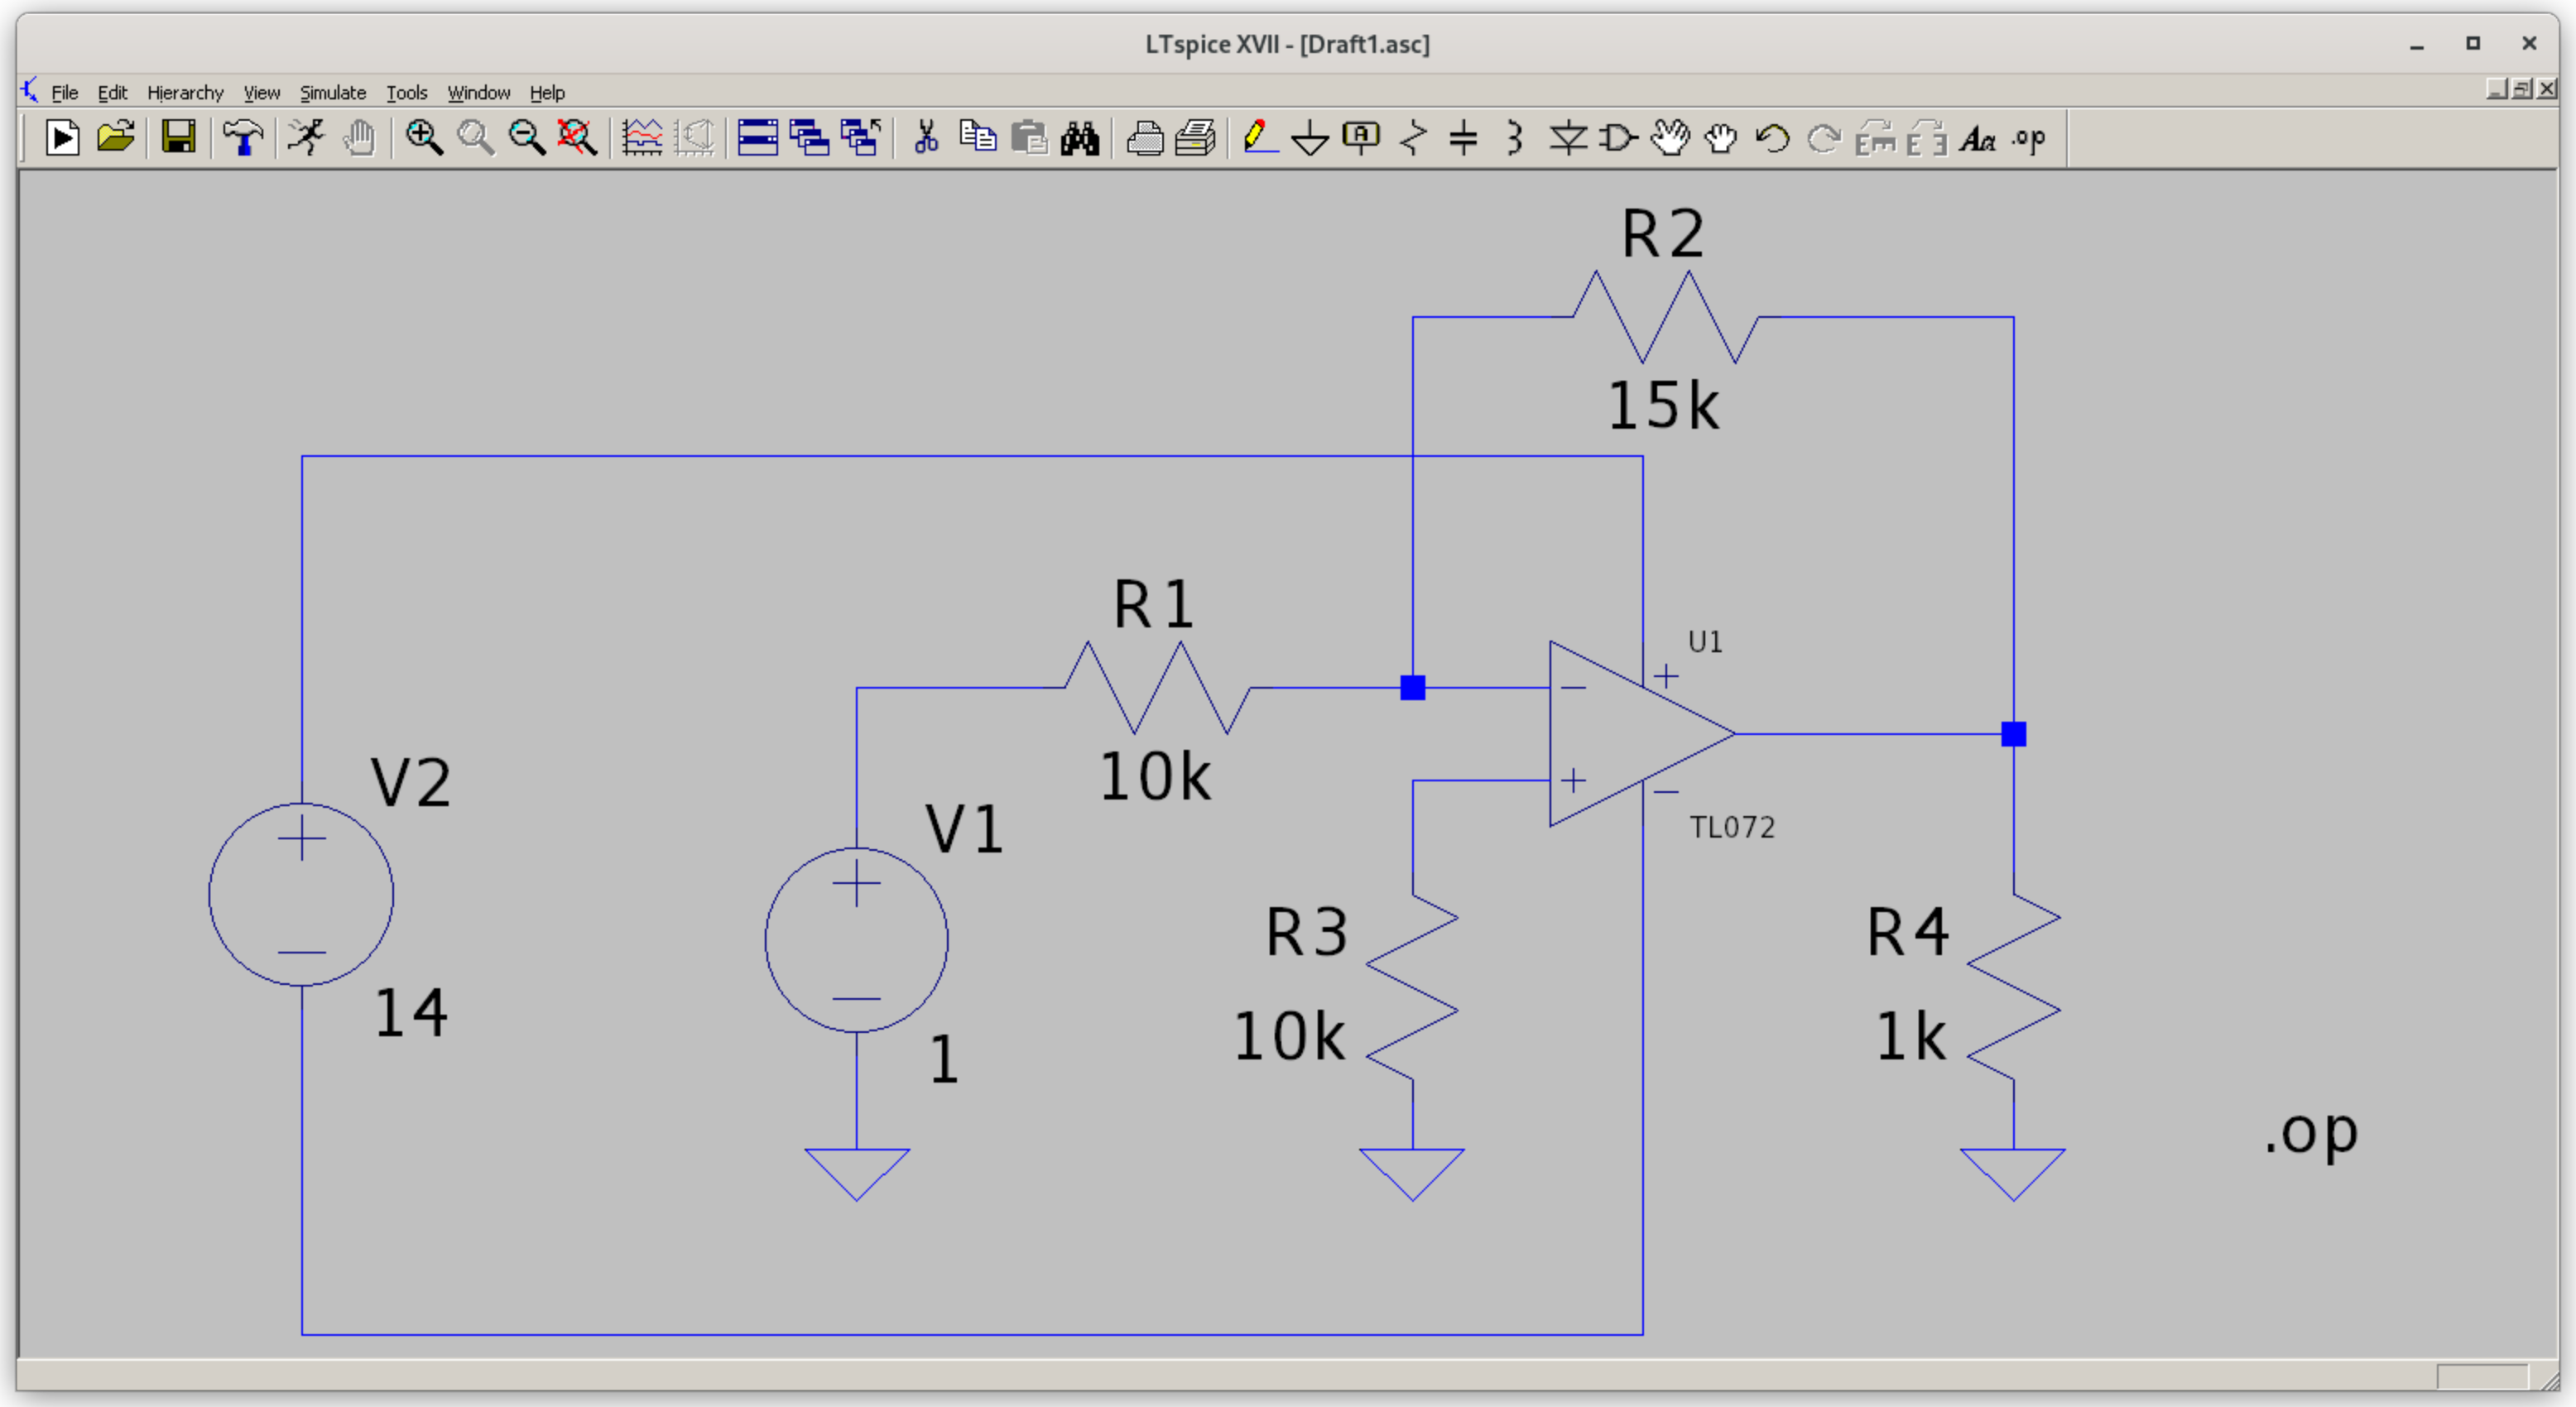
\includegraphics[width=0.8\textwidth]{img/1/ltspice.png}
    \caption{Pantalla de LTSpice}
    \label{fig:1:ltspice}
\end{figure}

\begin{table}[H]
    \centering
    \begin{tabular}{@{}r|rrrr@{}}
    \toprule
    $R_L$ (\si{\kilo\ohm}) & $v_o$ (\si{\volt}) & $v_+$ (\si{\nano\volt}) & 
    $v_-$ (\si{\milli\volt}) & $v_+ - v_-$ (\si{\milli\volt}) \\
    \midrule
    $47$ & $-13.6573$ & $-562.558$ & $-62.9007$ & $62.9001$ \\
    $10$ & $-13.5672$ & $-562.558$ & $-62.8992$ & $62.8986$ \\
     $1$ & $-13.6572$ & $-562.557$ & $-62.8821$ & $62.8815$ \\ \bottomrule
    \end{tabular}
    \caption{Tensiones según LTSpice ($v_i = \SI{9.00}{\volt}$)}
    \label{tab:1:ltspice-tensiones}
\end{table}

\begin{table}[H]
    \centering
    \begin{tabular}{@{}r|rrrr@{}}
        \toprule
        $R_L$ (\si{\kilo\ohm}) & $I_{R_1}$ (\si{\milli\ampere}) &
        $I_{R_2}$ (\si{\milli\ampere}) & $I_{R_3}$ (\si{\pico\ampere}) &
        $I_{R_L}$ (\si{\milli\ampere}) \\
        \midrule
        $47$ & $0.29058$ & $0.906290$ & $56.2558$ & $0.29058$ \\
        $10$ & $1.36572$ & $0.906290$ & $56.2558$ & $1.36572$ \\
         $1$ & $13.6572$ & $0.906288$ & $56.2557$ & $13.6572$ \\ \bottomrule
        \end{tabular}
        \caption{Corrientes según LTSpice}
        \label{tab:1:ltspice-corrientes}
\end{table}



\subsection{Datos obtenidos}

Se miden los siguientes valores de resistencias:

\begin{itemize}
        \input{src/1/snippets/resistencias}
\end{itemize}

Los valores medidos de $R_L$, comparados con sus valores nominales, se encuentran en la tabla \ref{tab:1-datos:resistencias-l}.

También se toman mediciones de las distintas tensiones presentes en el circuito (tablas \ref{tab:1-datos:tensiones-1} y \ref{tab:1-datos:tensiones-2}) que son utilizadas para calcular las corrientes que circulan por cada resistor y cuyos valores se encuentran en la tabla \ref{tab:1-datos:corrientes}.

\begin{table}[H]
    \centering
    \begin{tabular}{@{}rr@{}}
        \toprule
        $R_L$ (nominal, \si{\kilo\ohm}) & $R_L$ (medido, \si{\kilo\ohm})  \\
        \midrule
        \input{src/1/tables/resistencias-l}
    \end{tabular}
    \caption{Valores medidos de $R_L$}
    \label{tab:1-datos:resistencias-l}
\end{table}

\begin{table}[H]
    \centering
    \begin{tabular}{@{}rrrrrr@{}}
        \toprule
        $R_L$ (\si{\kilo\ohm}) & $v_i$ (\si{\volt}) & $v_o$ (\si{\volt}) & 
            $v_+$ (\si{\milli\volt}) & $v_-$ (\si{\milli\volt}) &
            $v_+ - v_-$ (\si{\milli\volt}) \\
        \midrule
        \input{src/1/tables/tensiones-1}
    \end{tabular}
    \caption{Tensiones medidas en el circuito (parte 1)}
    \label{tab:1-datos:tensiones-1}
\end{table}

\begin{table}[H]
    \centering
    \begin{tabular}{@{}rrrrrr@{}}
        \toprule
        $R_L$ (\si{\kilo\ohm}) & $V_{R_1}$ (\si{\volt}) & $V_{R_2}$ (\si{\volt})& $V_{R_3}$ (\si{\milli\volt}) & $V_{R_L}$ (\si{\volt}) \\
        \midrule
        \input{src/1/tables/tensiones-2}
    \end{tabular}
    \caption{Tensiones medidas en el circuito (parte 2)}
    \label{tab:1-datos:tensiones-2}
\end{table}

\begin{table}[H]
    \centering
    \begin{tabular}{@{}rrrrr@{}}
        \toprule
        $R_L$ (\si{\kilo\ohm}) & $I_{R_1}$ (\si{\milli\ampere}) & $I_{R_2}$ (\si{\milli\ampere}) & $I_{R_3}$ (\si{\nano\ampere}) & $I_{R_L}$ (\si{\milli\ampere}) \\
        \midrule
        \input{src/1/tables/corrientes}
    \end{tabular}
    \caption{Corrientes calculadas en el circuito}
    \label{tab:1-datos:corrientes}
\end{table}

La ganancia del operacional puede calcularse experimentalmente con las
ecuaciones \ref{ec:1-teoria:ganancia-experimental} y
\ref{ec:1-teoria:err-ganancia-experimental}. Los resultados de esta
operación se encuentran en la tabla \ref{tab:1-teoria:ganancia-experimental}.

\begin{equation}
    \label{ec:1-teoria:ganancia-experimental}
    A = \frac{v_o}{v_i}
\end{equation}

\begin{equation}
    \label{ec:1-teoria:err-ganancia-experimental}
    \Delta A = \left| \frac{1}{v_i} \right| \Delta v_o + \left| -\frac{v_o}{{v_i}^2} \right| \Delta v_i
\end{equation}

\begin{table}[H]
    \centering
    \begin{tabular}{@{}rr@{}}
        \toprule
        $R_L$ (\si{\kilo\ohm}) & $A$ \\
        \midrule
        \input{src/1/tables/ganancia-experimental}
    \end{tabular}
    \caption{Valores experimentales de ganancia}
    \label{tab:1-teoria:ganancia-experimental}
\end{table}

Teniendo $R_L = \SI{1}{\kilo\ohm}$ se reemplaza la pila de \SI{9}{\volt} por
un generador de funciones configurado para entregar una señal senoidal de
\SI{2}{\volt} de amplitud pico-a-pico y frecuencia $f = \SI{1}{\kilo\hertz}$.
Se conecta también un osciloscopio, cuya pantalla
se muestra en la fig. \ref{fig:1-datos:osciloscopio}. Se observa que la señal
de salida tiene una amplitud muy cercana a la de entrada (\SI{1.02}{\volt} vs.
\SI{1.08}{\volt}), y que se encuentra desfasada en unos \SI{90}{\degree}.

\begin{figure}[H]
    \centering
    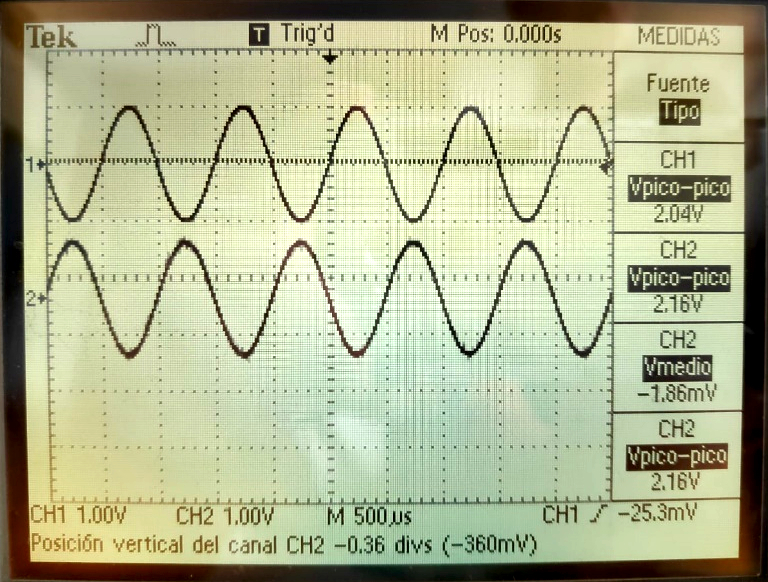
\includegraphics[width=0.8\textwidth]{img/1/osciloscopio-1.jpg}
    \caption{Pantalla del osciloscopio. Se muestran la señal de entrada
        (arriba, canal 1) y la de salida (abajo, canal 2).}
    \label{fig:1-datos:osciloscopio}
\end{figure}


\newpage
\subsection{Análisis de datos}

El gráfico de la fig. \ref{fig:1-analisis:ganancia} muestra una comparación
entre el valor de ganancia teórico (calculado con las ecuaciones 
\ref{ec:1-teoria:ganancia} y \ref{ec:1-teoria:err-ganancia}) y aquellos 
medidos en la práctica para los distintos valores de resistencia. Como puede
observarse, todos los valores de ganancia medidos caen cómodamente dentro
del margen de error previsto. Esto sugiere que las ecuaciones de ganancia
que se utilizaron para la configuración inversora del amplificador operacional
permiten obtener una buena aproximación al funcionamiento real del circuito.

\begin{figure}[H]
    \centering
    \input{img/1/ganancia.tikz}
    \caption{Valores de ganancia medidos vs. teóricos}
    \label{fig:1-analisis:ganancia}
\end{figure}

Dado que los valores medidos de tensión en la terminal no inversora son
mayores que $0$ en dos de los tres casos estudiados\footnote{Es altamente
probable que $v_+$ estuviera en el orden de los \si{\micro\volt}, en cuyo
caso nos fue imposible medir con el multímetro del que disponíamos.}, se
comprueba la explicación ofrecida en la sección \ref{sec:1-teoria} sobre la
utilización del resistor $R_3$. Si la resistencia de entrada del operacional
fuera infinita, esta tensión sería 0.


% \subsection{Análisis de datos}

La fig. \ref{fig:1-analisis:ganancia} compara la ganancia teórica con los valores obtenidos en la práctica.

\begin{figure}[H]
    \includegraphics[width=\textwidth]{img/1-analisis-ganancia.eps}
    \caption{Ganancia teórica vs. ganancia experimental}
    \label{fig:1-analisis:ganancia}
\end{figure}



    \newpage
    \section{Segunda parte: amplificador no inversor}

Se arma el circuito de la fig. \ref{fig:2:esquema} en un \textit{protoboard}
con $R_1 = \SI{10}{\kilo\ohm}$ y $R_2 = \SI{15}{\kilo\ohm}$, un TL072 como
amplificador operacional y una fuente partida de $\SI{14}{\volt}$
alimentándolo, además de una pila de \SI{9}{\volt} como $V_1$.
Luego se utilizan distintos valores de resistencia $R_L$
(47, 10 y \SI{1}{\kilo\ohm}) y se miden las tensiones $v_i$ y $v_o$ para
calcular la ganancia del circuito.

Hecho esto, se modifica el circuito para convertirlo en el seguidor de tensión
de la fig. \ref{fig:2:esquema-seguidor} (ver sección
\ref{sec:intro:opamp-noinversor}) y se vuelven a utilizar los
mismos valores de $R_L$ para hallar los distintos puntos de trabajo.

\begin{figure}[H]
    \centering
    \begin{subfigure}[b]{0.45\textwidth}
        \centering
        \begin{circuitikz}
    \node[op amp] at (0, 0) (opamp) {};

    \draw(opamp.+) -- ++(-0.2, 0) node[label={left:$v_+ = v_i$}]{}
    to[battery1, a=$V_1$] ++(0, -2) coordinate(cg)
    node[ground]{};

    \draw(opamp.-) -- ++(-0.7, 0) node[label={above:$v_-$}]{}
    to[R, a=$R_1$] ++(-1.5, 0)
    to[short] ++(-0.2, 0) coordinate(ci)
    to[short] (cg -| ci) node[ground]{};

    \draw(opamp.-) -- ++(-0.2, 0)
    to[short, *-] ++(0, 2)
    to[R=$R_2$] ++(2.8, 0) coordinate(co)
    to[short] (opamp.out -| co) coordinate(co1) -- (opamp.out);

    \draw(co1) 
    to[short, *-o] ++(0.4, 0) node[right]{$v_o$};

    \draw(co1)
    to[R=$R_L$] (cg -| co1) node[ground]{};

    \draw(opamp.up) -- ++(0, 0.2) node[vcc]{$+V_{cc}$};
    \draw(opamp.down) -- ++(0, -0.2) node[vee]{$-V_{cc}$};
\end{circuitikz}

        \caption{Amplificador no inversor}
        \label{fig:2:esquema}
    \end{subfigure}
    \hfill
    \begin{subfigure}[b]{0.45\textwidth}
        \centering
        \begin{circuitikz}
    \node[op amp] at (0, 0) (opamp) {};

    \draw(opamp.+) -- ++(-0.2, 0) node[label={below:$v_+$}]{}
    to[R=$R_1$] ++(-2, 0) node[label={above:$v_i$}]{}
    to[battery1, a=$V_1$] ++(0, -2) coordinate(cg)
    node[ground]{};

    \draw(opamp.-) node[label={left:$v_-$}]{};

    \draw(opamp.-) -- ++(-0.2, 0)
    to[short] ++(0, 2)
    to[R=$R_2$] ++(2.8, 0) coordinate(co)
    to[short] (opamp.out -| co) coordinate(co1) -- (opamp.out);

    \draw(co1) 
    to[short, *-o] ++(0.4, 0) node[right]{$v_o$};

    \draw(co1)
    to[R=$R_L$] (cg -| co1) node[ground]{};

    \draw(opamp.up) -- ++(0, 0.2) node[vcc]{$+V_{cc}$};
    \draw(opamp.down) -- ++(0, -0.2) node[vee]{$-V_{cc}$};
\end{circuitikz}

        \caption{Amplificador seguidor de tensión}
        \label{fig:2:esquema-seguidor}
    \end{subfigure}
    \caption{Circuitos a implementar}
\end{figure}

\subsection{Resolución teórica}

El circuito de la fig. \ref{fig:2:esquema} es prácticamente idéntico al de
la fig. \ref{fig:intro:opamp-no-inversor}, con el agregado del resistor $R_L$
que no modifica el valor de la tensión de salida.

Si se utiliza el modelo ideal planteado en la sección
\ref{sec:intro}, se puede despreciar el efecto del resistor
$R_1$ en el circuito de la fig. \ref{fig:2:esquema-seguidor}, ya que no
circulará corriente por esta rama debido a la alta resistencia de entrada del
operacional. De esta forma se obtiene el mismo circuito de la fig.
\ref{fig:intro:opamp-no-inversor}, con resistencia infinita entre la terminal
inversora y masa.

Para ambos casos, entonces, se puede utilizar la ec.
\ref{ec:intro:opamp-noinversor}. Al propagar el error se obtiene nuevamente
la ec. \ref{ec:1-teoria:err-ganancia}, motivo por el cual se obtiene una 
ganancia $A = \num{2.5 \pm 0.15}$ para el caso del amplificador no inversor,
y $A = \num{1.0}$ para el seguidor de tensión (incertidumbre nula, puesto que
$R_1 = \infty$).


\subsection{Simulación con LTSpice}

La simulación de LTSpice de la fig. \ref{fig:2:ltspice} del amplificador no
inversor de la fig. \ref{fig:2:esquema} arrojó una ganancia $A = 2.304$ en
todos los casos, que concuerda con el análisis teórico. El único factor que
varió fue la corriente $I_{R_L}$, de $0.4413$, $2.074$ y
$\SI{20.74}{\milli\ampere}$ para las resistencias de $47$, $10$ y 
$\SI{1}{\kilo\ohm}$.

Para el amplificador seguidor de tensión se simuló el circuito de la fig.
\ref{fig:2:esquema-seguidor} con LTSpice, según lo indicado en la fig.
\ref{fig:2:ltspice-seguidor}. En todos los casos se obtuvo una ganancia $A=0.998$, que
concuerda con lo visto en la sección anterior. La única variable que presentó
diferencias según el valor de $R_L$ que se utilizara fue, por supuesto, la 
corriente por dicho resistor, de $0.1911$, $0.8984$ y
$\SI{8.984}{\milli\ampere}$ para resistencias de $47$, $10$ y
$\SI{1}{\kilo\ohm}$, respectivamente.

\begin{figure}[H]
    \centering
    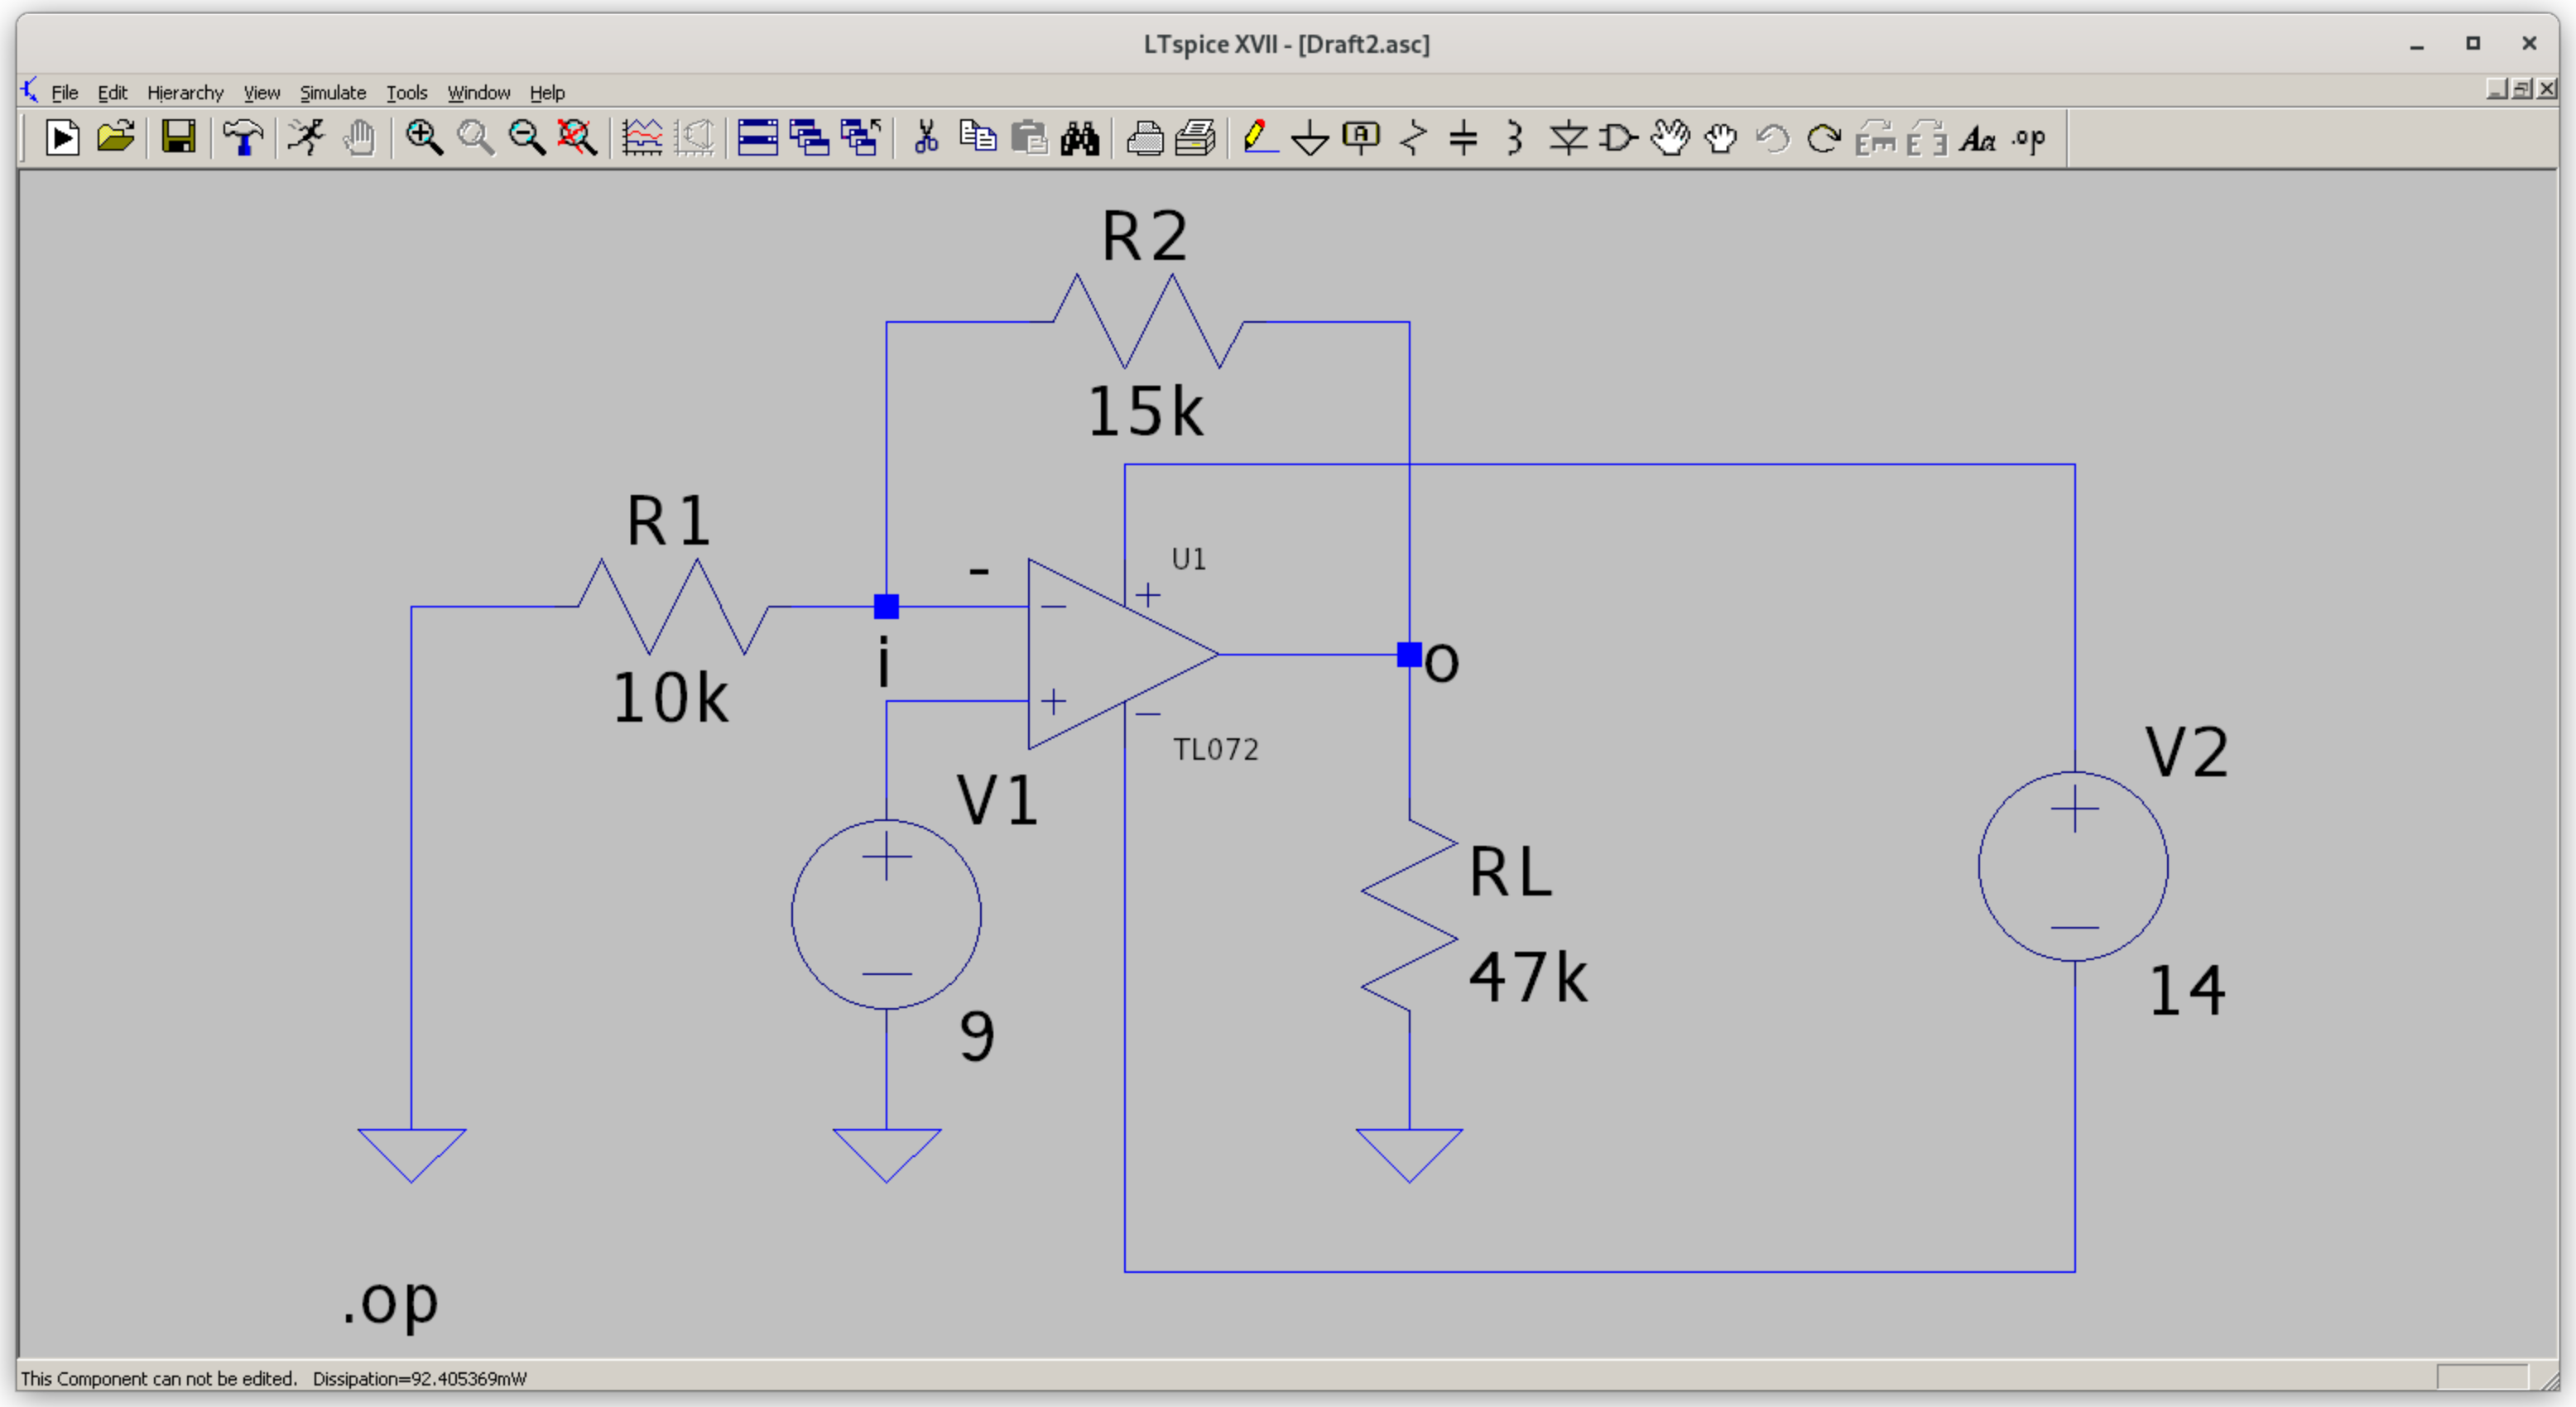
\includegraphics[width=0.8\textwidth]{img/2/ltspice.png}
    \caption{Simulación en LTSpice del circuito de la fig. \ref{fig:2:esquema}}
    \label{fig:2:ltspice}
\end{figure}

\begin{figure}[H]
    \centering
    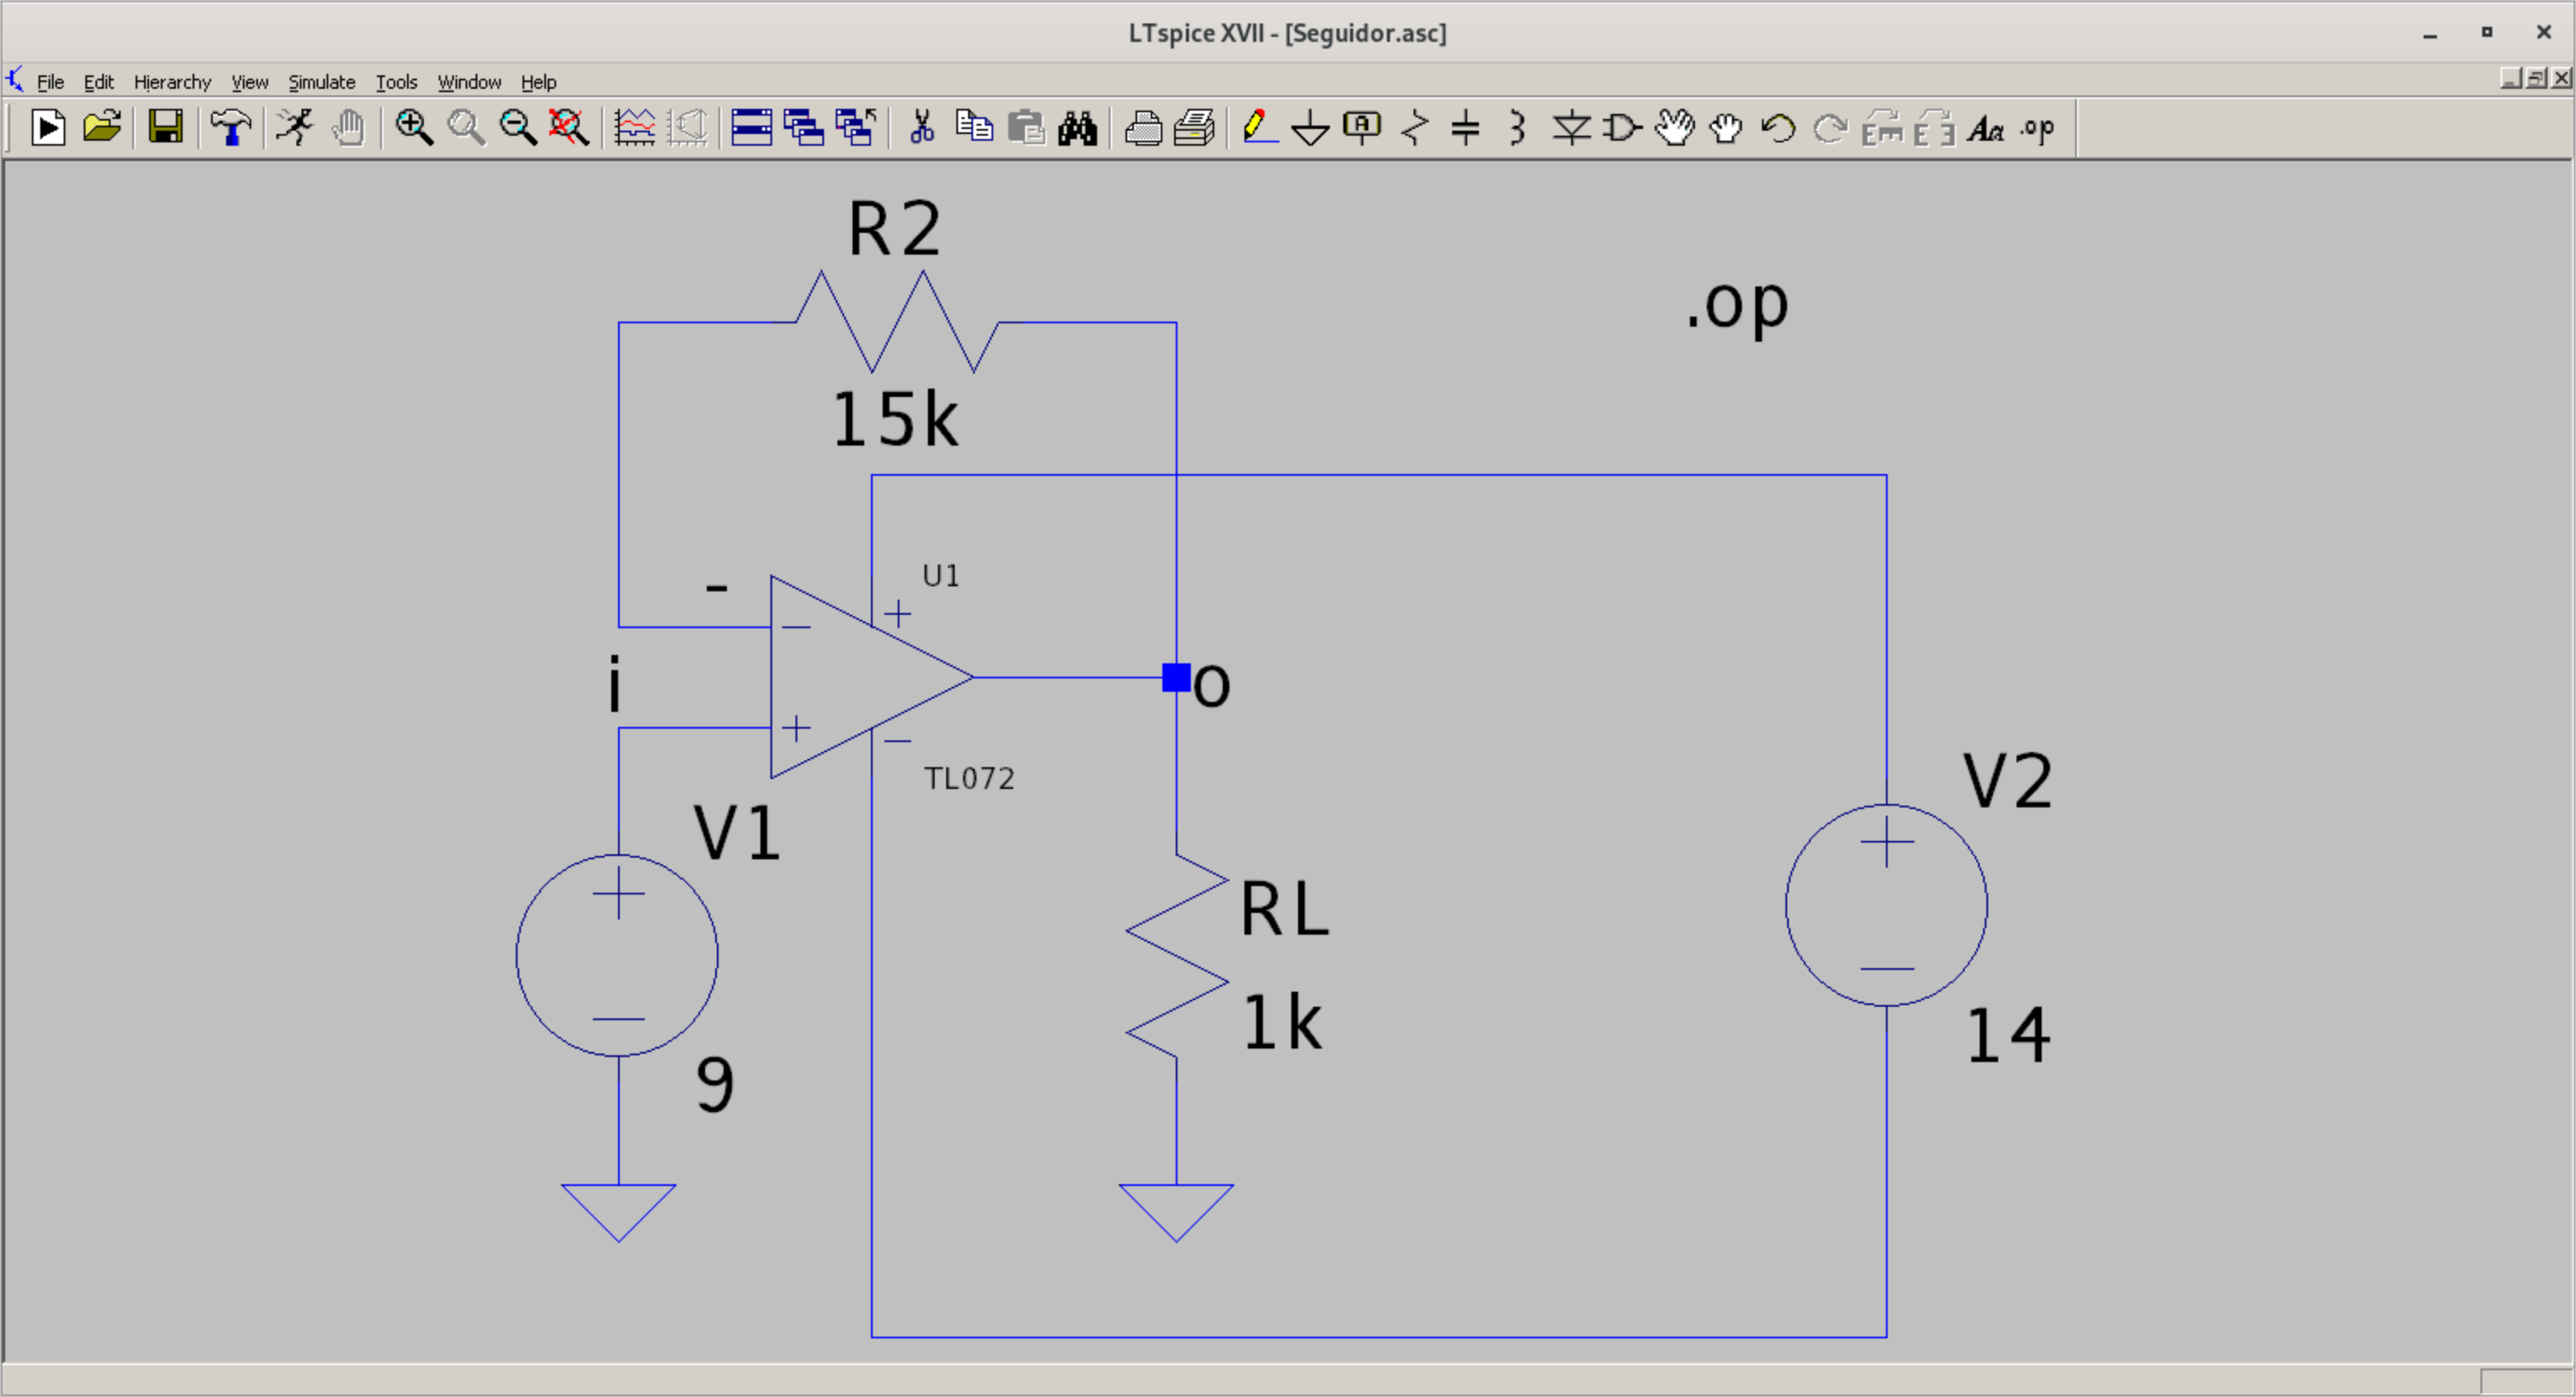
\includegraphics[width=0.8\textwidth]{img/2/ltspice-seguidor.png}
    \caption{Simulación en LTSpice del circuito de la fig.
        \ref{fig:2:esquema-seguidor}}
    \label{fig:2:ltspice-seguidor}
\end{figure}


\TODO{Agregar datos obtenidos, análisis y gráficos}


    \TODO{Agregar conclusiones}
    
    \newpage
    \section{Bibliografía}
    \printbibliography[heading=none]

\end{document}
